\documentclass[t,aspectratio=169]{beamer}

\usetheme{Frankfurt}
\usecolortheme{orchid}

\usepackage[T1]{fontenc}
\usepackage[utf8]{inputenc}
\usepackage{lmodern}
\usepackage{amsmath}
\usepackage{graphicx}
\usepackage{textcomp}
\usepackage{hyperref}
\usepackage{soul}
\usepackage{color}
\usepackage{tabularx}
\usepackage{colortbl}

\newif\ifcomplete
%\completetrue % comment out for the short presentation (ICPF version)

\title{ICFP Programming Contest 2014 -- Supermassive Black Hom-set Post-mortem}
\author{P. Lepin}
\date{}

\begin{document}

\frame{\titlepage}

\ifcomplete

\section{Silly Stuff}

\begin{frame}
  \frametitle{What's up with the name?}
  \begin{itemize}
    \item Time pressure -- wanted to submit ASAP, needed \textit{some} team name.
    \item<2-> Last year I played as \textquotedblleft{By Wadler's Beard!}\textquotedblright{ }Should have kept it.
  \end{itemize}
\end{frame}

\fi

\section{Overview}

\begin{frame}
  \frametitle{The Plan}
  Coding directly in GCC assembly possible, but painful. So...
  \begin{enumerate}
    \only<2>{\item Implement the VM.}
    \only<3->{\item \st{Implement the VM.} -- there was a web-based implementation}
    \only<2>{\item Write a parser for a stand-alone HLL or implement an eDSL.}
    \only<3->{\item Write a parser for a stand-alone HLL \st{or implement an eDSL.}}
    \only<2>{\item Implement static checks and/or optimizations.}
    \only<3->{\item \st{Implement static checks and/or optimizations.}}
    \only<2->{\item Implement codegen.}
    \only<2>{\item ...?}
    \only<3->{\item \st{...?}}
    \only<2->{\item \textbf{(end goal)} Implement the Lambda-Man AI.\newline}
    \item<4-> Implement symbolic labels on top of GHC assembly.
    \item<4-> \textbf{(end goal)} Implement a Ghost AI (or several).
  \end{enumerate}
  \only<5>{...some of these decisions were extremely myopic.}
\end{frame}

\begin{frame}
  \frametitle{Perceived Fun Factor}
  \begin{center}
    \begin{tabularx}{0.6\textwidth}{|X|c|c|}
      \hline
      & Tools & AI \\
      \hline
      Lambda-Man & \cellcolor{green!75}\textbf{FUN!} & \cellcolor{green!75}\textbf{FUN!} \\
      \hline
      Ghosts & \cellcolor{green!9}Less fun. & \cellcolor{green!9}Less fun. \\
      \hline
    \end{tabularx}
  \end{center}
  Lisp-machine CPU, compilers, fairly sophisticated AIs -- interesting. 8-bit CPUs and severely resource-constrained programs -- not so much.
\end{frame}

\begin{frame}
  \frametitle{Effort}
  \begin{center}
    \begin{tabularx}{0.8\textwidth}{|X|c|p{0.3\textwidth}|}
      \hline
      & Tools & \multicolumn{1}{c|}{AI} \\
      \hline
      Lambda-Man & \cellcolor{green!27}\textbf{\char`\~9 hrs}, 205 sloc & \cellcolor{green!75}\textbf{\char`\~25 hrs}, 654 sloc, 3114 instructions compiled \\
      \hline
      Ghosts & \cellcolor{green!9}\textbf{\char`\~3 hrs}, 259 sloc & \cellcolor{green!9}\textbf{\char`\~3 hrs}, 91 instruction \\
      \hline
    \end{tabularx}
  \end{center}
\end{frame}

\begin{frame}
  \frametitle{Wild Guesstimate Of Impact}
  \begin{center}
    \begin{tabularx}{0.6\textwidth}{|X|c|c|}
      \hline
      & Tools & AI \\
      \hline
      Lambda-Man & \multicolumn{2}{c|}{\cellcolor{green!9}Some.} \\
      \hline
      Ghosts & \multicolumn{2}{c|}{\cellcolor{green!75}\textbf{HUGE!}} \\
      \hline
    \end{tabularx}
  \end{center}
  Judging by the results of home-brewed tournaments on reddit.
\end{frame}

\section{Gory Details}

\begin{frame}
  \frametitle{HLL Compiler Targetting GCC}
  \begin{itemize}
    \item HLL is Lisp-like, mimicking Scheme and Clojure.
    \only<2>{\begin{figure}[!h]
      \centering
      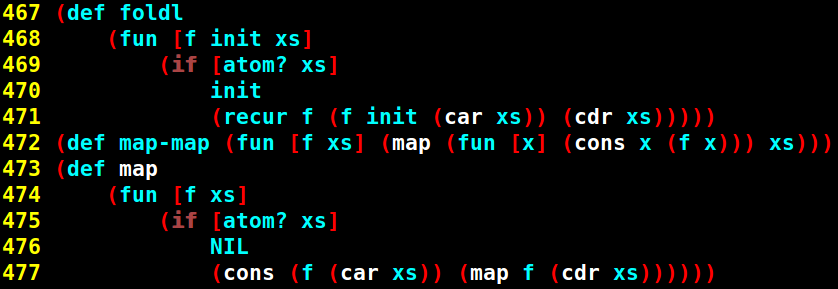
\includegraphics[width=0.8\textwidth]{scimitar}
      \caption{Almost looks like the real thing.}
    \end{figure}}
    \only<3->{\item Almost purely functional, \texttt{set!} is accepted by the parser, but... \only<5->{is not supported.}}
    \only<4>{\begin{figure}[!h]
      \centering
      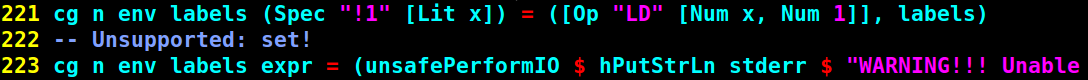
\includegraphics[width=0.8\textwidth]{noset}
      \caption{Not really supported.}
    \end{figure}}
    \only<5->{\item The only effectful part is \texttt{do}/\texttt{debug}.}
    \only<6->{\item \textbf{Many} quirks:
    \begin{itemize}
      \item<7-> No general TCE, explicit (and unchecked) tail recursion optimization using \texttt{recur}.
      \item<8-> Mildly insane function call convention to support \texttt{recur} -- incompatible with ABI as in spec.
      \item<9-> \texttt{if}s must be in a tail position - no support for \texttt{SEL}.
      \item<10-> Built-ins such as \texttt{car} or \texttt{+} are special forms rather than first-class entities.
      \item<11-> No macros.
      \item<12-> Virtually no diagnostics or static checks -- a pain to debug.
    \end{itemize}}
    \only<13->{\item Implementing as eDSL could have given some type safety \textit{almost for free}.}
  \end{itemize}
\end{frame}

\begin{frame}
  \frametitle{HLL Compiler Targetting GCC -- Bugs}
  \begin{itemize}
    \item A couple of nasty bugs \char`\~30 hrs into the contest.
    \only<2->{\begin{figure}[!h]
      \centering
      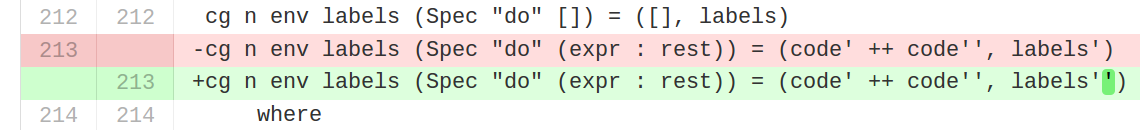
\includegraphics[width=0.64\textwidth]{typecheck}
      \caption{The fact that it typechecks doesn't \textit{always} mean it's correct.
      (But encoding the codegen in a monad \textit{could} have helped.)}
    \end{figure}}
    \only<3>{\begin{figure}[!h]
      \centering
      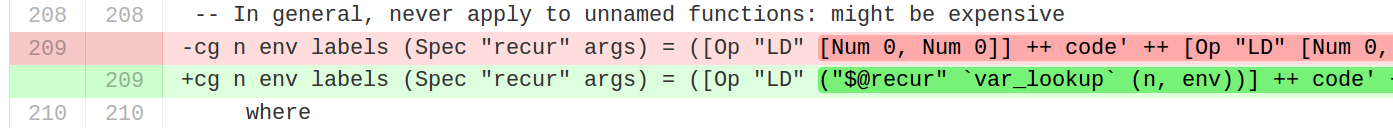
\includegraphics[width=0.8\textwidth]{recur}
      \caption{\texttt{recur} only worked -- occasionally -- by accident.}
    \end{figure}}
  \end{itemize}
\end{frame}

\begin{frame}
  \frametitle{Lambda-Man AI}
  \begin{itemize}
    \item Lightning round AI retained as a fall-back -- main AI may not return a move in situations it considers hopeless:
    \begin{itemize}
      \item Manhattan distance to the closest pill as a value function.
      \item Doesn't like being too close to ghosts or visiting recently seen locations (reduces the effect of local minima).
    \end{itemize}
    \only<2->{\item BFS: cuts off on dying, reaching anything edible or exceeding the depth limit.}
    \only<3-5>{\begin{itemize}
      \item<3-5> Being close to ghosts is penalized.
      \item<4-5> If nothing edible found, simple heuristic value function kicks in.
      \item<5> Likes running towards nearest power pill when ghosts are nearby.    
    \end{itemize}}
    \only<6->{\item Data structures: binary search trees (logarithmic access map and IntSet), simple queue from \textit{PFDS}.}
    \only<7>{\begin{figure}[!h]
      \centering
      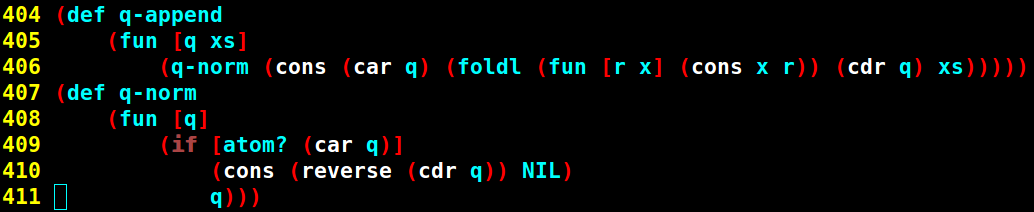
\includegraphics[width=0.8\textwidth]{pfds}
    \end{figure}}
    \only<8->{\item Propagates ghosts (ignoring differences in speed) as long as they have no choice.}
    \only<9>{\begin{figure}[!h]
      \centering
      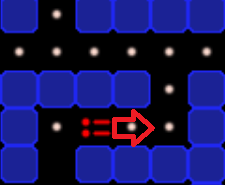
\includegraphics[width=0.1\textwidth]{ghostprop-init}
      \caption{Initial state.}
    \end{figure}}\only<10>{\begin{figure}[!h]
      \centering
      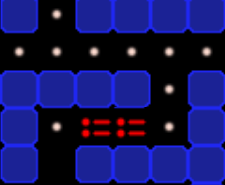
\includegraphics[width=0.1\textwidth]{ghostprop-1}
      \caption{After 1 step.}
    \end{figure}}\only<11>{\begin{figure}[!h]
      \centering
      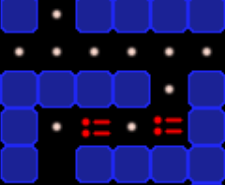
\includegraphics[width=0.1\textwidth]{ghostprop-2}
      \caption{After 2 steps.}
    \end{figure}}\only<12>{\begin{figure}[!h]
      \centering
      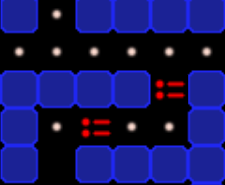
\includegraphics[width=0.1\textwidth]{ghostprop-3}
      \caption{After 3 steps.}
    \end{figure}}\only<13>{\begin{figure}[!h]
      \centering
      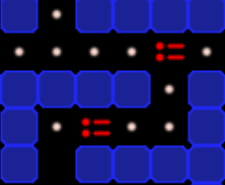
\includegraphics[width=0.1\textwidth]{ghostprop-4}
      \caption{After 4 or more steps.}
    \end{figure}}
    \only<14->{\item Value of scared ghosts and fruits discounted by time to expiration.}
  \end{itemize}
\end{frame}

\begin{frame}
  \frametitle{Lambda-Man AI -- Quirks}
  \begin{itemize}
    \item Termination of search on reaching anything edible leads to \textquotedblleft{interesting}\textquotedblright{ }behavior.
    \item<2-> Scaredy Lambda-Man -- pessimistic estimates of ghost movement.
    \item<3-> Very little global preprocessing -- computing tunnels as graph edges was tempting.
    \item<4-> Unnecessary map preprocessing on each step.
    \item<5-> AI state fragile -- failures screw up future behavior.\newline
    \item<6-> \textbf{Not-a-quirk:} Ghost AIs known, but emulation impractical due to cycle limit.
  \end{itemize}
\end{frame}

\begin{frame}
  \frametitle{Lambda-Man AI -- Panic}
  \begin{itemize}
    \item A few hours before the deadline...
    \only<2>{\begin{figure}[!h]
      \centering
      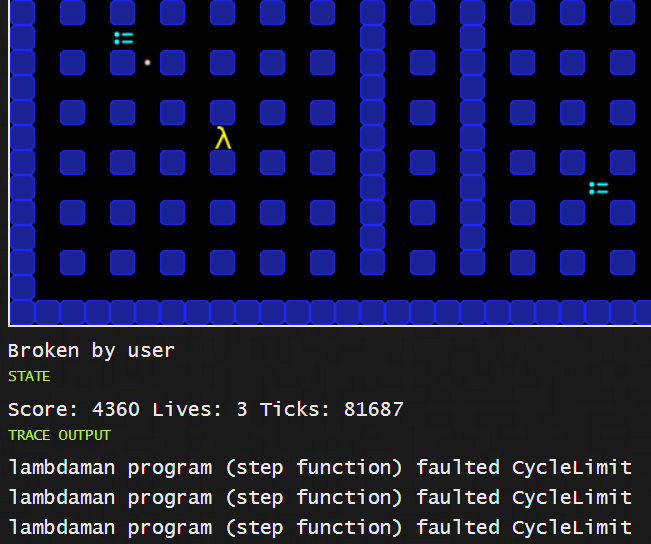
\includegraphics[width=0.4\textwidth]{cycle-limit}
      \caption{OMG!!! Cycle limit!}
    \end{figure}}
    \only<3->{\item Hard to estimate cycles spent sanely from inside the simulation.}
    \only<4->{\item Regretted not having my own VM -- web implementation sluggish \textit{and} read-only.}
    \only<5>{\begin{figure}[!h]
      \centering
      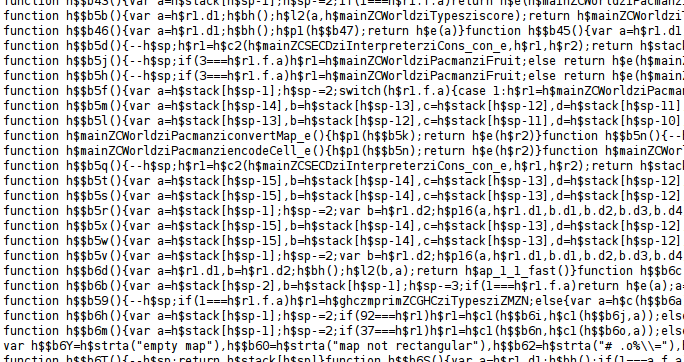
\includegraphics[width=0.5\textwidth]{goodluck}
      \caption{Good luck editing \textit{this}.}
    \end{figure}}
    \only<6->{\item Regretted not having macros -- no easy inlining.}
    \only<7->{\item Random BFS depth cutoffs based on the map size.}
    \only<8->{\item Optimized by hand.
    \begin{itemize}
      \item<9-> Non-tail recursive list HOFs -- no artifical limitations on stack depth, \texttt{RTN}s are cheaper than reversing the accumulator.
      \only<9>{\begin{figure}[!h]
        \centering
        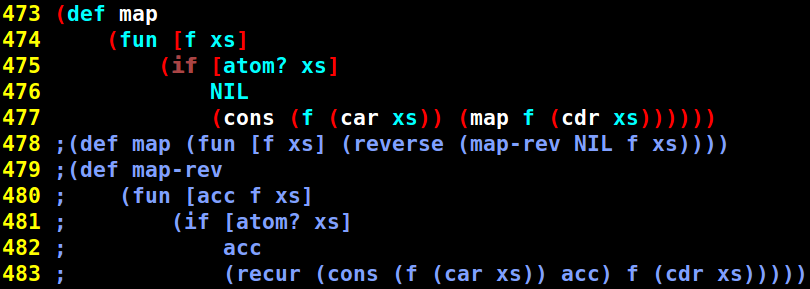
\includegraphics[width=0.5\textwidth]{nontailrec}
      \end{figure}}
      \item<10-> Fused \texttt{map}s and \texttt{filter}s in a few places.
      \item<11-> Eliminated some unneeded intermediate variables.
    \end{itemize}}
    \only<12->{\item Seems to have worked.}
  \end{itemize}
\end{frame}

\begin{frame}
  \frametitle{Ghost AI}
  \begin{itemize}
    \item \textit{Very} limited resources -- even accounting for no need to make decisions on most runs.
    \only<2->{\item Wanted something simple and reasonably robust.}
    \only<3->{\item Tries to minimize $L_1$ distance to Lambda-Man (\textit{Blinky}/\textit{Chaser}-style).}
    \only<4-5>{\begin{itemize}
      \item<4-5> \textbf{Problem:} Ghosts tend to clump together.
      \item<5> \textbf{Problem:} Can get stuck in dead ends easily.
    \end{itemize}}
    \only<6->{\item Ghost's index affects tie-breaks: different ghosts favour different directions at intersections.}
    \only<7->{\item Simple counter: after a few actual decisions in a row resulting in horizontal or vertical move, that axis is excluded.}
    \only<8->{\item Pretty efficient on non-pathological maps: ghosts tend to surround the Lambda-Man.}
  \end{itemize}
\end{frame}

\begin{frame}
  \frametitle{Sources}
  \begin{itemize}
    \item Submission is available on GitHub, link can be found on ICFPC subreddit, along with many interesting submissions and reports from other teams:
    \url{http://www.reddit.com/r/icfpcontest}
  \end{itemize}
\end{frame}

\ifcomplete

\section{Lessons (Un)Learned}

\begin{frame}
  \frametitle{How To Win The ICFP Programming Contest}
  \framesubtitle{What I learned from past failures and how I used it this time -- or not}
  \begin{itemize}
    \only<1-2>{\item Try to decipher the hint.
    \only<2>{\begin{figure}[!h]
      \centering
      
\includegraphics[width=0.3\textwidth]{bkg}
      \caption{The apparently black background image on the official site has slight brightness variations. This \textquotedblleft{steganographic message}\textquotedblright{ }turned out to be random noise. D'oh!}
    \end{figure}}}
    \only<3->{\item \st{Try to decipher the hint.}}
    \only<4-7>{\item Do your research.
      \begin{itemize}
        \item<5-7> There are people smarter than I am on the Net.
        \item<6-7> SECD -- little insight into the problem, the spec was enough.
        \item<7> Classic ghost AIs -- could have mislead me.
      \end{itemize}}
    \only<8->{\item \st{Do your research.}}
    \only<9-11>{\item If you want to do well -- get on a strong team.
      \begin{itemize}
        \item<10-11> But can be stressful.
        \item<11> And I'm in it for the sheer fun of it...
      \end{itemize}}
    \only<12->{\item \st{If you want to do well -- get on a strong team.}}
    \only<13-14>{\item Don't forget to rest, eat and sleep. \only<14>{On the other hand...}}
    \only<15->{\item \st{Don't forget to rest, eat and sleep.}}
    \only<16-17>{\item Random tweaks don't work. Think instead.
    \only<17>{\begin{figure}[!h]
      \centering
      
\includegraphics[width=0.9\textwidth]{tweak}
      \caption{Cutoff depth selection for BFS. Speaks for itself.}
    \end{figure}}}
    \only<18->{\item \st{Random tweaks don't work. Think instead.}}
    \only<19-21>{\item Read the spec carefully.
      \begin{itemize}
        \item<20-21> Signed my submissions with SHA256 instead of SHA1.
        \item<21> Only noticed minutes before the deadline.
      \end{itemize}}
    \only<22->{\item \st{Read the spec carefully.}}
    \only<23-25>{\item Use C++.
      \begin{itemize}
        \item<24-25> It appears to dominate the field as far as the tools of choice for discriminating hackers are concerned.
        \item<25> Used Haskell this year.
      \end{itemize}}
    \only<26->{\item \st{Use C++.}}
    \only<27->{\item All in all, I have no idea how does this work.}
  \end{itemize}
\end{frame}

\section{Shout-outs}

\begin{frame}
  \frametitle{Lots of teams from Eastern Europe and Russia for some reason?}
  \begin{itemize}
    \item<1-> In 2012 the organizers expressed puzzlement with a somewhat skewed geographical distribution of teams.
    \item<2-> Dmitry Astapov's ICFPC reports (\url{http://users.livejournal.com/_adept_/tag/icfpc}) -- in Russian
    \item<3-> Better reading than most fiction.
    \item<4-> The 2006 one stands out in particular (and so did the contest itself).
    \item<5-> Many folks who read those reports were instantly hooked and wanted to give it a shot -- myself included.
    \item<6-> Now you know whom to blame.
  \end{itemize}
\end{frame}

\begin{frame}
  \frametitle{Compilers Are Scary Stuff}
  \begin{itemize}
    \item<1-> Considered to be a dark art among the uninitiated.
    \item<2-> Dr. Alex Aiken and his team are running an open Compilers class on Coursera -- \url{https://www.coursera.org/course/compilers}
    \item<3-> It's a good one. Get through it and you'll never be scared of writing a compiler again.
    \item<4-> \textbf{Correction:} writing a \textit{toy} compiler.
    \item<5-> Thankfully, the GHC and GCC in this contest were not the Real Thing.
  \end{itemize}
\end{frame}

\begin{frame}
  \frametitle{AI Is A Bit Scary Too}
  \begin{itemize}
    \item<1-> Dr. Dan Klein and others developed an Artificial Intelligence class on edX -- \url{https://www.edx.org/course/uc-berkeleyx/uc-berkeleyx-cs188-1x-artificial-579}
    \item<2-> Curiously, it uses Pac-Man in examples and assignments a lot.
    \begin{figure}[!h]
      \centering
      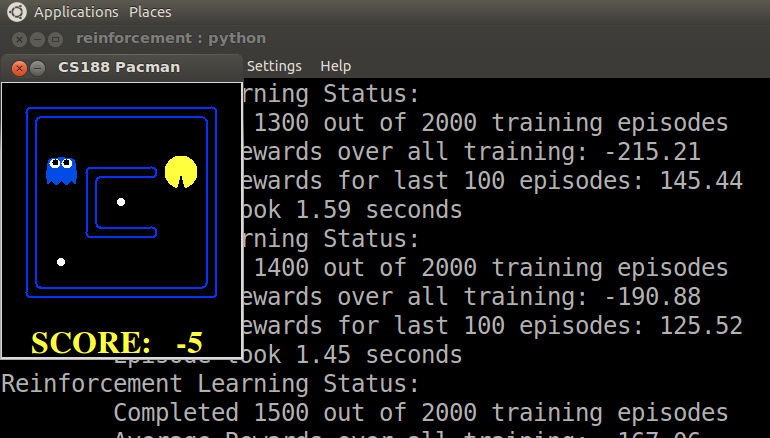
\includegraphics[width=0.3\textwidth]{cs188}
    \end{figure}
    \item<3-> I'm sure that's sheer coincidence and had \textit{nothing} to do with my performance here.
  \end{itemize}
\end{frame}

\fi

\begin{frame}[c]
  \begin{center}
    \textbf{This was even more awesome than ICFP contests usually are.}
  
    \textbf{Heartfelt thanks to the organizers.}
    
    \textbf{And thank you for listening.}
  \end{center}
\end{frame}

\ifcomplete

\begin{frame}[c]
  \begin{center}
    \textbf{And remember -- for the next year, Haskell is the programming tool of choice for discriminating hackers.}
  \end{center}
\end{frame}

\fi

\end{document}
